\documentclass[notes,11pt, aspectratio=169]{beamer}

\usepackage{pgfpages}
% These slides also contain speaker notes. You can print just the slides,
% just the notes, or both, depending on the setting below. Comment out the want
% you want.
\setbeameroption{hide notes} % Only slide
%\setbeameroption{show only notes} % Only notes
%\setbeameroption{show notes on second screen=right} % Both

\usepackage{helvet}
\usepackage[default]{lato}
\usepackage{array}
\usepackage{tgbonum}

\usepackage{tikz}
\usepackage{verbatim}
\setbeamertemplate{note page}{\pagecolor{yellow!5}\insertnote}
\usetikzlibrary{positioning}
\usetikzlibrary{snakes}
\usetikzlibrary{calc}
\usetikzlibrary{arrows}
\usetikzlibrary{decorations.markings}
\usetikzlibrary{shapes.misc}
\usetikzlibrary{matrix,shapes,arrows,fit,tikzmark}
\usepackage{amsmath}
\usepackage{mathpazo}
\usepackage{hyperref}
\usepackage{lipsum}
\usepackage{multimedia}
\usepackage{graphicx}
\usepackage{multirow}
\usepackage{graphicx}
\usepackage{dcolumn}
\usepackage{bbm}
\newcolumntype{d}[0]{D{.}{.}{5}}

\usepackage{changepage}
\usepackage{appendixnumberbeamer}
\newcommand{\beginbackup}{
   \newcounter{framenumbervorappendix}
   \setcounter{framenumbervorappendix}{\value{framenumber}}
   \setbeamertemplate{footline}
   {
     \leavevmode%
     \hline
     box{%
       \begin{beamercolorbox}[wd=\paperwidth,ht=2.25ex,dp=1ex,right]{footlinecolor}%
%         \insertframenumber  \hspace*{2ex}
       \end{beamercolorbox}}%
     \vskip0pt%
   }
 }
\newcommand{\backupend}{
   \addtocounter{framenumbervorappendix}{-\value{framenumber}}
   \addtocounter{framenumber}{\value{framenumbervorappendix}}
}


\usepackage{graphicx}
\usepackage[space]{grffile}
\usepackage{booktabs}
\newcommand\independent{\protect\mathpalette{\protect\independenT}{\perp}}
\def\independenT#1#2{\mathrel{\rlap{$#1#2$}\mkern2mu{#1#2}}}
\DeclareMathOperator{\Supp}{Supp}

% These are my colors -- there are many like them, but these ones are mine.
\definecolor{blue}{RGB}{0,114,178}
\definecolor{red}{RGB}{213,94,0}
\definecolor{yellow}{RGB}{240,228,66}
\definecolor{green}{RGB}{0,158,115}

\hypersetup{
  colorlinks=false,
  linkbordercolor = {white},
  linkcolor = {blue}
}


%% I use a beige off white for my background
\definecolor{MyBackground}{RGB}{255,253,218}

%% Uncomment this if you want to change the background color to something else
%\setbeamercolor{background canvas}{bg=MyBackground}

%% Change the bg color to adjust your transition slide background color!
\newenvironment{transitionframe}{
  \setbeamercolor{background canvas}{bg=yellow}
  \begin{frame}}{
    \end{frame}
}

\setbeamercolor{frametitle}{fg=blue}
\setbeamercolor{title}{fg=black}
\setbeamertemplate{footline}[frame number]
\setbeamertemplate{navigation symbols}{}
\setbeamertemplate{itemize items}{-}
\setbeamercolor{itemize item}{fg=blue}
\setbeamercolor{itemize subitem}{fg=blue}
\setbeamercolor{enumerate item}{fg=blue}
\setbeamercolor{enumerate subitem}{fg=blue}
\setbeamercolor{button}{bg=MyBackground,fg=blue,}



% If you like road maps, rather than having clutter at the top, have a roadmap show up at the end of each section
% (and after your introduction)
% Uncomment this is if you want the roadmap!
% \AtBeginSection[]
% {
%    \begin{frame}
%        \frametitle{Roadmap of Talk}
%        \tableofcontents[currentsection]
%    \end{frame}
% }
\setbeamercolor{section in toc}{fg=blue}
\setbeamercolor{subsection in toc}{fg=red}
\setbeamersize{text margin left=1em,text margin right=1em}

\newenvironment{wideitemize}{\itemize\addtolength{\itemsep}{10pt}}{\enditemize}

\usepackage{environ}
\NewEnviron{videoframe}[1]{
  \begin{frame}
    \vspace{-8pt}
    \begin{columns}[onlytextwidth, T] % align columns
      \begin{column}{.70\textwidth}
        \begin{minipage}[t][\textheight][t]
          {\dimexpr\textwidth}
          \vspace{8pt}
          \hspace{4pt} {\Large \sc \textcolor{blue}{#1}}
          \vspace{8pt}

          \BODY
        \end{minipage}
      \end{column}%
      \hfill%
      \begin{column}{.38\textwidth}
        \colorbox{green!20}{\begin{minipage}[t][1.2\textheight][t]
            {\dimexpr\textwidth}
            Face goes here
          \end{minipage}}
      \end{column}%
    \end{columns}
  \end{frame}
}

\pgfdeclareimage[height=\paperheight]{mybackground}{images/diff_in_diff.png}


\setbeamertemplate{title page}{

        \begin{picture}(0,0)

            \put(-11,-150){%
                \pgfuseimage{mybackground}
            }

            \put(0,-50.7){%
                \begin{minipage}[b][45mm][t]{226mm}
                    \usebeamerfont{title}{\inserttitle\par}
                \end{minipage}
            }

            \end{picture}

    }


\title[]{\textcolor{blue}{Canonical Research Designs I:\\ Difference-in-Differences:\\ Basics, Pre-trends, and Inference}}
\author[PGP]{}
\institute[FRBNY]{\small{\begin{tabular}{c}
  Paul Goldsmith-Pinkham  \\
\end{tabular}}}

\date{\today}

\begin{document}

%%% TIKZ STUFF
\tikzset{
	every picture/.style={remember picture,baseline},
	every node/.style={anchor=base,align=center,outer sep=1.5pt},
	every path/.style={thick},
}
\newcommand\marktopleft[1]{%
	\tikz[overlay,remember picture]
	\node (marker-#1-a) at (-.3em,.3em) {};%
}
\newcommand\markbottomright[2]{%
	\tikz[overlay,remember picture]
	\node (marker-#1-b) at (0em,0em) {};%
}
\tikzstyle{every picture}+=[remember picture]
\tikzstyle{mybox} =[draw=black, very thick, rectangle, inner sep=10pt, inner ysep=20pt]
\tikzstyle{fancytitle} =[draw=black,fill=red, text=white]
%%%% END TIKZ STUFF

% Title Slide
\begin{frame}
	\maketitle
\end{frame}

\begin{frame}{Revisiting Research Design}
	\begin{columns}[T] % align columns
		\begin{column}{0.8\textwidth}
			\begin{wideitemize}
				\item Recall my attempt at a definition:
				\begin{itemize}
					\item A \emph{(causal) research design} is a statistical and/or economic
					      statement of how an empirical research paper will estimate a
					      relationship between two (or more) variables that is causal in nature: how $X$ causes $Y$.
				\end{itemize}
				\item Recall these research designs can be considered into two types:
				\begin{itemize}
					\item \emph{Model}-based: the estimand is identified using
					      assumptions on the modeling of the potential outcomes
					      conditional on treatment and additional variables
					      \item\emph{Design}-based: the estimand is
					      identified using assumptions on the treatment variable,
					      conditional on the potential outcomes and additional
					      variables
				\end{itemize}
			\end{wideitemize}
		\end{column}%
		\hfill%
		\begin{column}{.5\textwidth}
		\end{column}%
	\end{columns}
\end{frame}


\begin{frame}{Revisiting Research Design}
	\begin{columns}[T] % align columns
		\begin{column}{0.7\textwidth}
			\begin{wideitemize}
				\item The design-based ideal is not necessarily achievable in all scenarios
				\item Recall the reason for wanting a randomized experiment: we want to estimate \emph{counterfactual} outcomes
				\item Alternative way to do this: model the outcome (absent treatment) directly
				\begin{itemize}
					\item The relationship between X and Y can be clearly
					      articulated, but the ``experimental design'' analogy is more fraught/complicated
				\end{itemize}
				\item This issue will become clear as we discuss our first topic
			\end{wideitemize}
		\end{column}%
		\hfill%
		\begin{column}{.7\textwidth}

		\end{column}%
	\end{columns}
\end{frame}


\begin{frame}{Estimating causal effects in real settings}
	\begin{columns}[T] % align columns
		\begin{column}{.58\textwidth}
			\begin{wideitemize}
				\item In many applications, we want to estimate the effect of a policy across groups
				\item However, the policy assignment is  \emph{not} necessarily uncorrelated with group characteristics
				\item How can we identify the effect of the policy without being confounded by these level differences?
			\end{wideitemize}
		\end{column}%
		\hfill%
		\begin{column}{.38\textwidth}
			{\onslide<2->
				\vspace{30pt}
				\begin{center}
					\Large \textcolor{red}{Difference-in-differences!}
					\normalsize (DinD)
				\end{center}
			}
		\end{column}%
	\end{columns}
\end{frame}

\begin{frame}{Difference-in-differences}
	\begin{columns}[T] % align columns
		\begin{column}{.5\textwidth}
			\begin{wideitemize}
				\item Difference-in-differences has become the dominant methodology
				for estimating causal effects in applied work
				\item True across all fields (Goldsmith-Pinkham (2024))
			\end{wideitemize}
		\end{column}%
		\hfill%
		\begin{column}{.5\textwidth}
			\vspace{-10pt}
			\begin{center}
				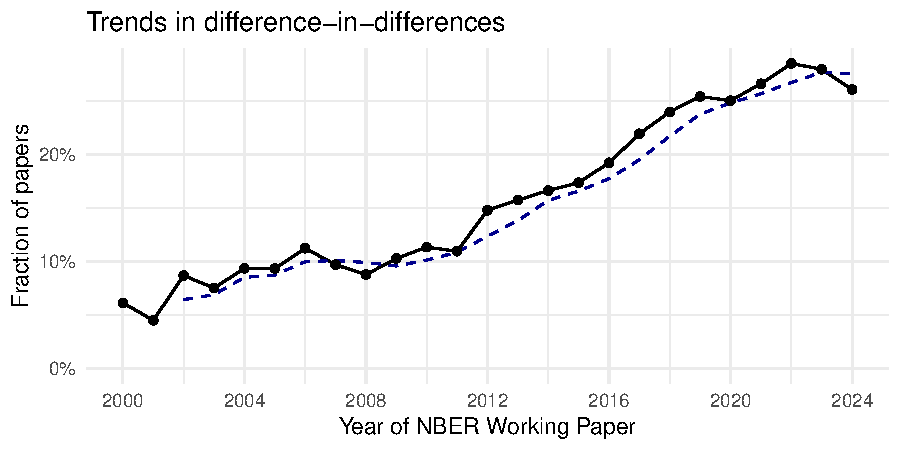
\includegraphics[width=\linewidth]{images/extend_results_didforguido.pdf}

				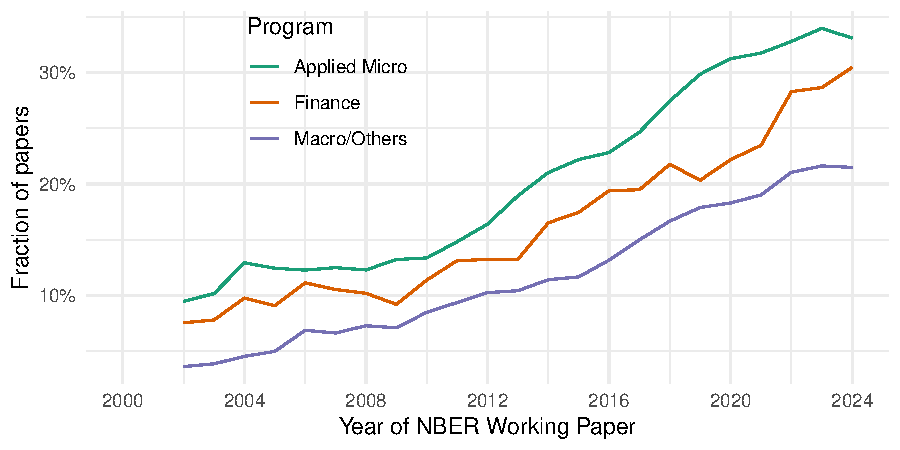
\includegraphics[width=\linewidth]{images/extend_results_didby_group.pdf}
			\end{center}
		\end{column}%
	\end{columns}
\end{frame}

\begin{frame}{First, a warning}
	\begin{columns}[T] % align columns
		\begin{column}{.99\textwidth}
			\begin{wideitemize}
				\item This literature has had a certain amount of upheaval over the
				past 5-6 years
				\item Tension: provide context for how people currently and
				historically have studied diff-in-diff
				\begin{itemize}
					\item But also elaborate on concerns identified in recent papers
				\end{itemize}
				\item The key issues boil down into two questions:
				\begin{enumerate}
					\item \emph{What is the counterfactual estimand?}
					      \begin{itemize}
						      \item Does your estimator map to your estimand? (e.g. ``Are you getting at what you meant to?'')
					      \end{itemize}
					\item \emph{What are your structural assumptions and their implications?}
					      \begin{itemize}
						      \item Do you need to assume functional forms?
					      \end{itemize}
				\end{enumerate}
				\item Papers have both pointed out issues but also provided
				solutions to almost all of the problems that they've raised,
				so not something that should prevent you from using these
				tools
			\end{wideitemize}
		\end{column}%
		\hfill%
		\begin{column}{.38\textwidth}

		\end{column}%
	\end{columns}
\end{frame}


\begin{frame}{Cases of DinD}
	\begin{columns}[T] % align columns
		\begin{column}{.58\textwidth}
			\begin{wideitemize}
				\item 1 treatment timing, Binary treatment, 2 periods
				\begin{itemize}
					\item Card and Krueger  (AER, 1994)
				\end{itemize}
				\item 1 treatment timing, Binary treatment, T periods
				\begin{itemize}
					\item Yagan (AER, 2015)
				\end{itemize}
				% \item 1 treatment timing, Continuous treatment
				%   \begin{itemize}
				%   \item Berger, Turner and Zwick (JF, 2020)
				%   \end{itemize}
				\item Staggered treatment timing, Binary treatment
				\begin{itemize}
					\item Bailey and Goodman-Bacon (AER, 2015)
				\end{itemize}
			\end{wideitemize}
		\end{column}%
		\hfill%
		\begin{column}{.38\textwidth}
			% \makebox[\linewidth][c]{
			% \resizebox{\linewidth}{!}{
			% \includegraphics{how-to-draw-an-owl.pdf}
			% }
			% }
		\end{column}%
	\end{columns}
\end{frame}


\begin{frame}{Simple setup in basic 2x2 Diff-in-diff }
	\begin{wideitemize}
		\item Assume we have $n$ units ($i$) and $T=2$ time periods ($t$)
		\item Consider a binary policy $D_{it}$, and we are interested
		in estimating its effect on outcomes $Y_{it}$
		\item Consider the potential outcome notation for $Y_{it}$:
		\begin{itemize}
			\item $Y_{it}(0,0)$ is the outcome in period $t\in \{1,2\}$ if untreated in both periods
			\item $Y_{it}(0,1)$ is the outcome in period $t\in \{1,2\}$ if
			      untreated in first period, treated in second
			\item Can simplify to just $Y_{it}(0)$ and $Y_{it}(1)$, but when
			      we have many time periods, want to account for path of treatments
		\end{itemize}
		\item The inherent problem is that $D_{it}$ is \emph{not}
		necessarily randomly assigned, but we still want to estimate the ATT in period 2:
		\begin{equation*}
			\tau_{2}^{ATT} = E(Y_{i,2}(1) - Y_{i,2}(0) | D_{i} = 1)
		\end{equation*}
	\end{wideitemize}
\end{frame}


\begin{frame}{Basic 2x2 DinD setup}
	\begin{columns}[T] % align columns
		\begin{column}{0.8\textwidth}
			\begin{wideitemize}
				\item Recall our typical estimand of interest is the ATE or the ATT:
				\begin{align*}
					\tau_{ATE} & = E(Y_{it}(1) - Y_{it}(0)) = E(\tau_{i})                          \\
					\tau_{ATT} & = E(Y_{it}(1) - Y_{it}(0) | D_{it} = 1) = E(\tau_{i} |D_{it} = 1)
				\end{align*}
				\item Since $D$ is not randomly assigned, this model is inherently not identified without the additional assumptions (and two time periods).
				\begin{itemize}
					\item Why? $D_{i}$ could be correlated with $\alpha_{i}$
					\item Recall that our plug-in estimator approaches need
					      estimates for $E(Y_{it}(1))$ and $E(Y_{it}(0))$
					\item But the correlation prevents this without conditional exogeneity assumptions
				\end{itemize}
				\item Using the assumptions and multiple time periods, we can make progress!
			\end{wideitemize}
		\end{column}%
		\hfill%
		\begin{column}{.45\textwidth}
		\end{column}%
	\end{columns}
\end{frame}


\begin{frame}{2 $\times$ 2 DinD estimation}
	\begin{center}
		\begin{tabular}{c|cc}
			        & t =0                                   & t = 1                                \\
			\midrule
			$D = 0$ & $\gamma_{0} + \alpha_{i}$              & $ \gamma_{1} + \alpha_{i}$           \\
			$D = 1$ & $ \gamma_{0} + \alpha_{i} + \tau_{i} $ & $\gamma_{1} + \alpha_{i} + \tau_{i}$
		\end{tabular}
	\end{center}
	\begin{wideitemize}
		\item Now consider the within unit difference:
		$$Y_{i1} - Y_{i0} = (\gamma_{1} - \gamma_{0}) + \tau_{i}(D_{i1} - D_{i0})$$
		\item Hence
		\begin{align*}
			E(Y_{i1} - Y_{i0} | D_{i1} - D_{i0} = 1) - E(Y_{i1} - Y_{i0} | D_{i1} - D_{i0} = 0) & = E(\tau_{i}  | D_{i1} - D_{i0} = 1)
		\end{align*}
		\item Wait, you say, that's a lot more notation than I was expecting.
		\begin{itemize}
			\item Simplifying assumption: treatment only goes one way in
			      period 1
			\item  ``absorbing adoption'', e.g. $D_{i0} = 0$
		\end{itemize}
		\begin{align*}
			E(Y_{i1} - Y_{i0} | D_{i1} = 1) - E(Y_{i1} - Y_{i0} | D_{i1} = 0) =  \underbrace{E(\tau_{i}  | D_{i1} = 1) }_{ATT}
		\end{align*}
	\end{wideitemize}
\end{frame}


\begin{frame}{Basic 2x2 Diff-in-diff}
	How can we identify the ATT?
	\begin{enumerate}
		\item Parallel Trends: ``in the absence of the treatment, the average outcomes would have evolved in parallel''
		      \begin{equation*}
			      E(Y_{i,2}(0) - Y_{i,1}(0) | D_{i} = 1) =     E(Y_{i,2}(0) - Y_{i,1}(0) | D_{i} = 0)
		      \end{equation*}
		      \begin{itemize}
			      \item Absent the policy, units may have different \emph{levels}, but their changes would be the same
			      \item A sufficient parametric formulation: $Y_{it}(0) = \gamma_{t} + \alpha_{i} + \epsilon_{it}$
		      \end{itemize}
		\item No-anticipation: policy has no effect prior to treatment
		      \begin{equation*}
			      E(Y_{i,1}(0)) = E(Y_{i,1}(1))
		      \end{equation*}
	\end{enumerate}
\end{frame}

\begin{frame}{Another way to see this, assuming absorbing treatment}
	\begin{wideitemize}
		\item Rewrite the parallel trends assumption:
		\begin{equation*}
			E(Y_{i,2}(0)| D_{i} = 1) =  E( Y_{i,1}(0) |D_{i} = 1) +   E(Y_{i,2}(0) - Y_{i,1}(0) | D_{i} = 0)
		\end{equation*}
		\item In other words, the counterfactual ``untreated'' state is
		the untreated outcome in the pre-period for the treated group,
		plus the change from the other untreated group
		\item Then, thanks to no-anticipation, we can replace
		$E( Y_{i,1}(0) |D_{i} = 1)$ with $E( Y_{i,1}(1) |D_{i} = 1)$,
		which has an empirical analog:
		\begin{equation*}
			E(Y_{i,2}(0)| D_{i} = 1) =  E( Y_{i,1} |D_{i} = 1) +   E(Y_{i,2} - Y_{i,1} | D_{i} = 0)
		\end{equation*}
		\item So parallel trends + no-anticipation generates our
		counterfactual outcome for us!
		\item Pop quiz: where does no-anticipation show up in the
		parametric formulation?
	\end{wideitemize}

\end{frame}

\begin{frame}{An aside on our simplifying assumption on absorbing treatment}
	\begin{wideitemize}
		\item The choice of focusing on take-up of a policy, such that $D_{i1} \geq D_{i0}$, is well-grounded in many policy settings
		\item However, there are cases where policies turn on, and then turn off, and this can vary across units
		\item This can be challenging and potentially problematic with
		heterogeneous effects
		\item De Chaisemartin and d'Haultfoeuille (2020) allow for this, but not innocuous
		\begin{itemize}
			\item Additional assumption required (will discuss in subsequent classes)
		\end{itemize}
		\item Is $D_{i}$ turning on identical (but opposite sign) to $D_{i}$
		turning off?
		\begin{itemize}
			\item Hull (2018) working paper on mover designs discusses this
		\end{itemize}
		\item For today, will ignore this issue
	\end{wideitemize}
\end{frame}

\begin{frame}{Estimation using linear regression}
	\begin{wideitemize}
		\item A simple linear regression will identify
		$E(\tau_{i} | D_{i1} = 1)$ with two time periods:
		\begin{equation}
			Y_{it} = \alpha_{i}+ \gamma_{t} + D_{it}\beta + \epsilon_{it}
		\end{equation}
		\item This setup is sometimes referred to as the Two-way Fixed Effects estimator (TWFE)
		\item Note: we could have also estimated $\tau$ directly:
		\begin{align*}
			\hat{\tau} = n^{-1}\sum_{i} \underbrace{D_{i}(Y_{i1} - Y_{i0})}_{\Delta \overline{Y}_{1}} - \underbrace{(1-D_{i1})(Y_{i1} - Y_{i0})}_{\Delta \overline{Y}_{0}}
		\end{align*}
		\begin{itemize}
			\item Intuitively, we generate a counterfactual for the treatment
			      using the changes in the untreated units: $E(Y_{i1} - Y_{i0} | D_{i}=0)$
		\end{itemize}
		\item Necessary condition: two time periods! What if we have more?
	\end{wideitemize}
\end{frame}

\begin{frame}{Card and Krueger (1994)}
	\begin{wideitemize}
		\item Card and Krueger (1994) study the impact of New Jersey
		increasing the minimum wage 4.25 to 5.05 dollars an hour on April
		1, 1992
		\item Key question is what impact does this have on employment?
		\begin{itemize}
			\item Need a counterfactual for NJ, and use Pennsyvania as a control
		\end{itemize}
		\item Collected data in 410 fast food restaurants
		\begin{itemize}
			\item Called places and asked for employment and starting wage data
			\item Sample data from Feb 1992 and Nov 1992
		\end{itemize}
		\item Hence, $D_{i}$ is NJ vs PA, and $t=0$ is Feb 1992 and $t = 1$ is Nov 1992
	\end{wideitemize}
\end{frame}

\begin{frame}{Stark Effect on Wages in Card and Krueger (1994) }
	\begin{center}
		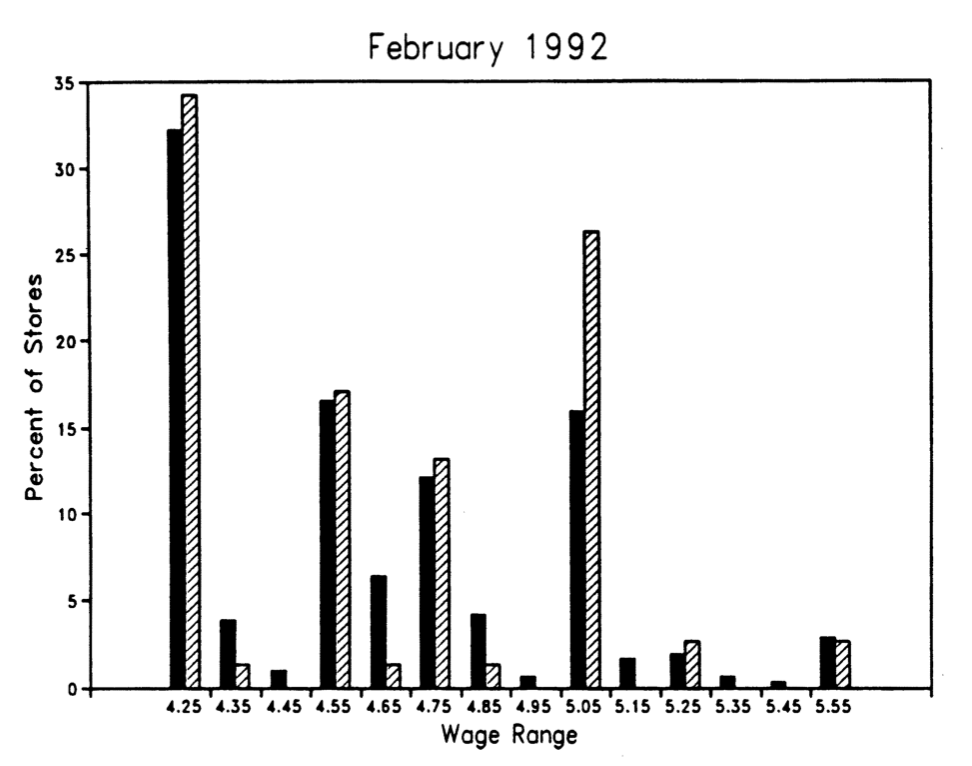
\includegraphics[width=0.45\linewidth]{images/cardkrueger1.png}   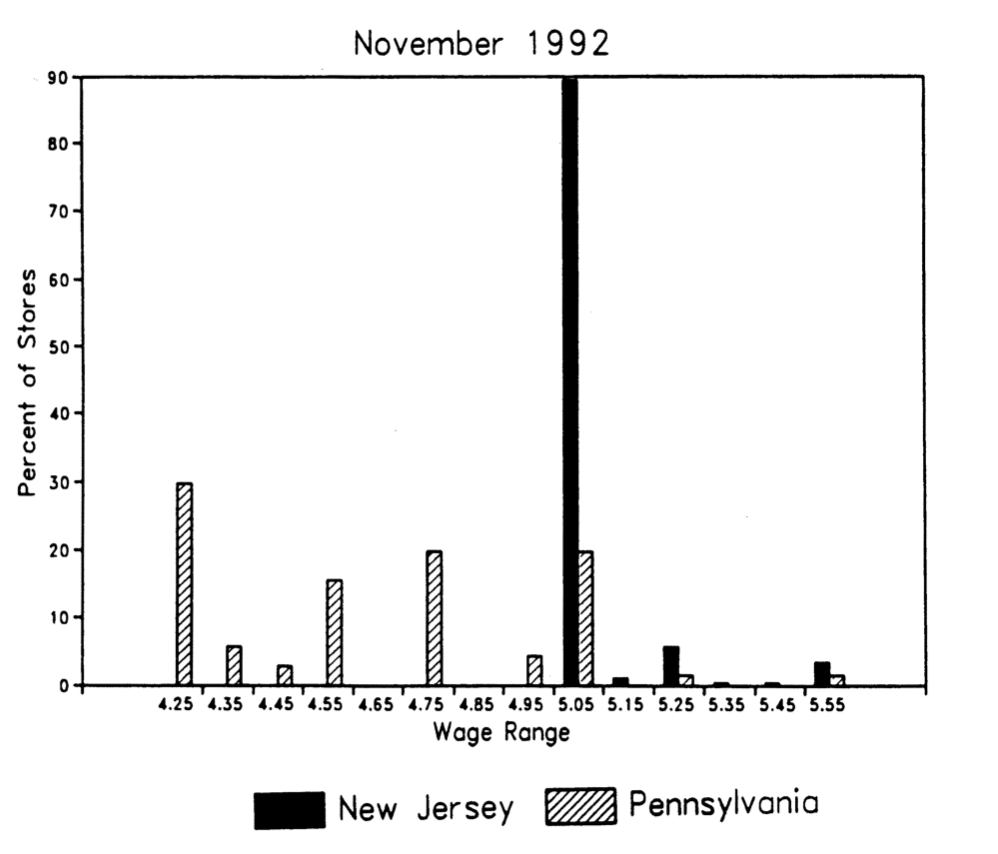
\includegraphics[width=0.45\linewidth]{images/cardkrueger2.png}
	\end{center}
\end{frame}


\begin{frame}{Effect on Employment in Card and Krueger (1994) }
	\begin{columns}[T] % align columns
		\begin{column}{0.5\textwidth}
			\begin{wideitemize}
				\item Despite a large increase in wages, seemingly no negative
				impact on employment
				\begin{itemize}
					\item In fact, marginally significant positive impact
				\end{itemize}
				\item Looking at raw data, this positive impact is driven by a
				decline in PA
				\begin{itemize}
					\item This decline is reasonable if you think that PA is a
					      good counterfactual, since 1992 is in the middle of a recession
				\end{itemize}
				\item A second comparison can be run with stores whose starting
				wage in pre-period was above treatment cutoff
				\begin{itemize}
					\item These stores perform similarly to PA
				\end{itemize}
			\end{wideitemize}
		\end{column}%
		\hfill%
		\begin{column}{.5\textwidth}
			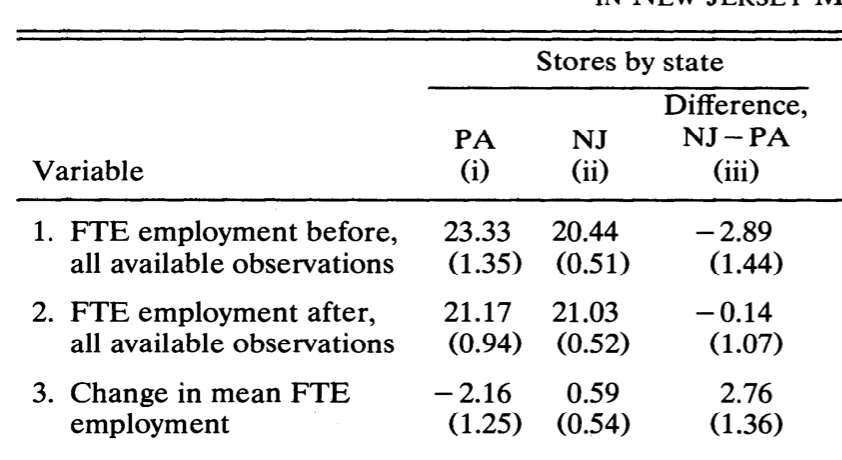
\includegraphics[width=\linewidth]{images/cardkrueger3.png}\\
			\hfill      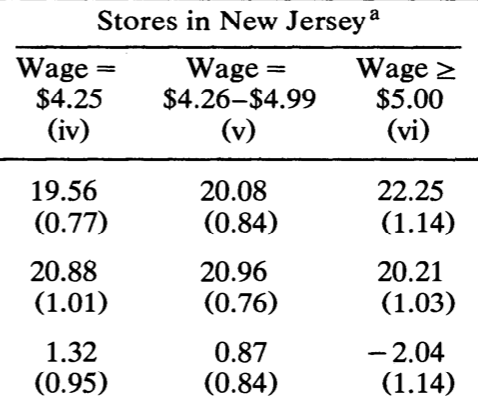
\includegraphics[width=0.5\linewidth]{images/cardkrueger4.png}
		\end{column}%
	\end{columns}
\end{frame}

\begin{frame}{Key considerations for thinking about Card and Krueger (1994)}
	\begin{wideitemize}
		\item The treatment can't really be thought of as randomly assigned
		\begin{itemize}
			\item Treatment is completely correlated within states
			\item As a result, any within-state correlation of errors will be
			      correlated with treatment status
		\end{itemize}
		\item Given the limited number of states, time periods, and
		treatments, more valuable to view this as a case study
		\begin{itemize}
			\item Under strong parametric assumptions, can infer causality!
			\item Card acknowledges (Card and Krueger interview with Ben Zipperer):
		\end{itemize}
		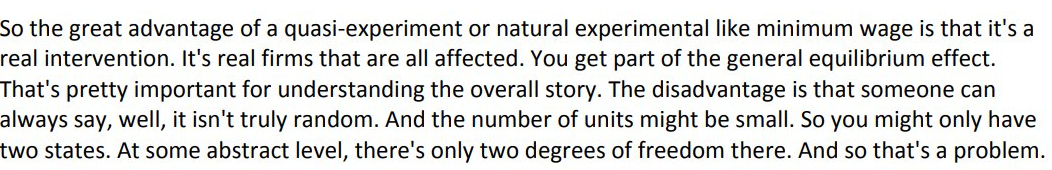
\includegraphics[width=\linewidth]{images/card_interview.png}
	\end{wideitemize}
\end{frame}

\begin{frame}{Multiple time periods in basic setup}
	\begin{wideitemize}
		\item Let's consider a policy that occurs all at $t_{0}$
		(e.g. single timing rolled out to treated units)
		\item  More time periods helps in several ways:
		\begin{enumerate}
			\item If we have multiple periods \emph{before} the policy implementation, we can partially test the underlying assumptions
			      \begin{itemize}
				      \item Sometimes referred to as ``pre-trends''
			      \end{itemize}
			\item If we have multiple periods \emph{after} the policy implementation, we can examine effect timing
			      \begin{itemize}
				      \item Is it an immediate effect? Does it die off? Is it persistent?
				      \item If you pool all time periods together into one ``post'' variable, this estimates the average effect. If sample is not balanced, can have unintended effects!
			      \end{itemize}
		\end{enumerate}
		\item  How do we implement this?
		\begin{equation*}
			Y_{it} = \alpha_{i} + \gamma_{t} + \sum_{t=1, t\not=t_{0}}^{T}\delta_{t} D_{it} + \epsilon_{it},
		\end{equation*}
		\begin{itemize}
			\item One of the coefficients is fundamentally unidentified
			      because of $\alpha_{i}$
			\item All coefficients measure the effect \emph{relative} to period $t_{0}$.
		\end{itemize}
	\end{wideitemize}
\end{frame}

\begin{frame}{Pre-testing and structural assumptions}
	\begin{wideitemize}
		\item Note that for the above model, we made a stronger assumption about trends
		\begin{itemize}
			\item We assumed that
			      $Y_{it}(d) - Y_{i,t-k}(d) = \gamma_{t} - \gamma_{t-k}$ for all
			      $k$ and $d$
			\item This is testable pre-treatment (hence the pre-test)
		\end{itemize}
		\item This is very powerful and has helped spark the growth in DinD regressions
		\begin{itemize}
			\item Visual demonstrate of ``pre-trends'' helps support the
			      validity of the design
			\item Worth doing!
		\end{itemize}
		\item Two key issues:
		\begin{enumerate}
			\item Pre-testing can cause statistical problems
			\item What does parallel trends even mean?
		\end{enumerate}
	\end{wideitemize}
\end{frame}

\begin{frame}{Pre-testing issues (Roth 2020)}
	\begin{columns}[T] % align columns
		\begin{column}{0.5\textwidth}
			\begin{wideitemize}
				\item Consider $T = 3$ and think about what a pre-trend test is
				trying to do
				\item Testing whether the difference relative to $t= 0$ for $t=-1$ is significant
				\item<3-> Unconditionally, this is reasonable. However, Roth
				(2020) highlights that this is a form of \emph{pre-testing},
				and that low power in detecting pre-trends can be problematic
				\item<5-> By selecting on pre-trends that ``pass'', will tend to
				choose baseline realizations that satisfy pre-trends, but
				induce \emph{bias} in the effect
			\end{wideitemize}
		\end{column}%
		\hfill%
		\begin{column}{.5\textwidth}
			\only<1>{      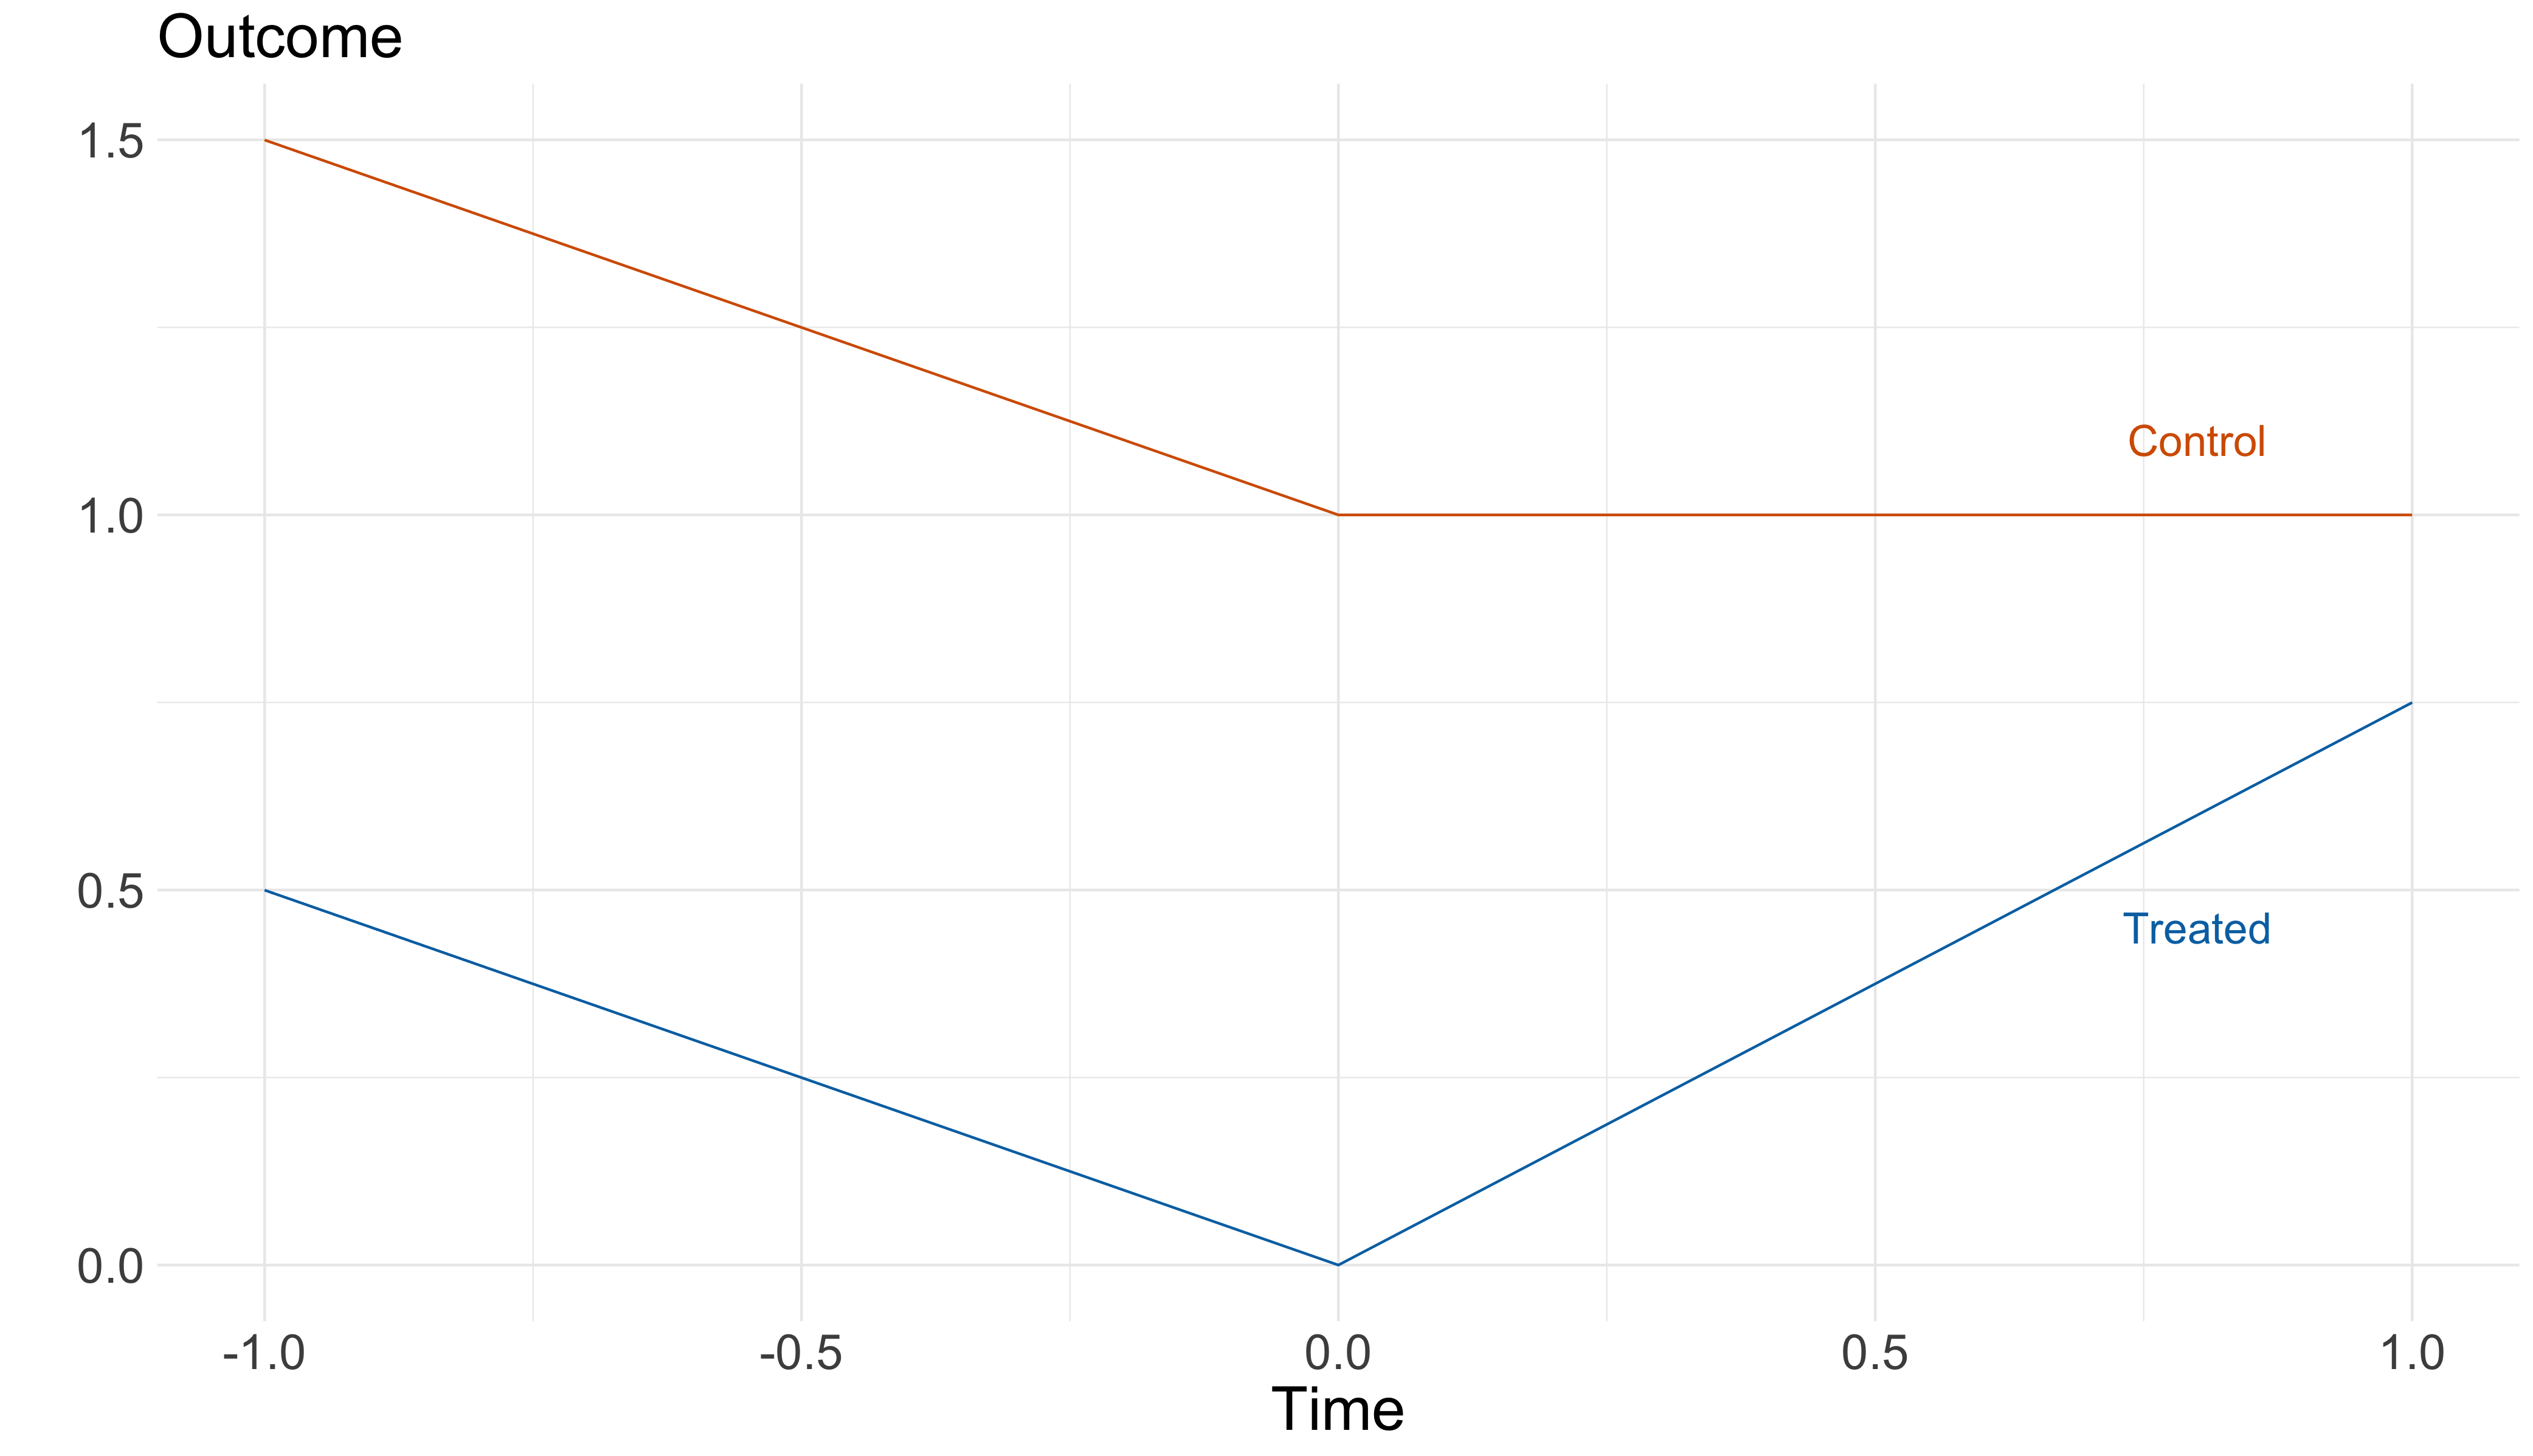
\includegraphics[width=\linewidth]{images/rothpic1.png}}
			\only<2>{      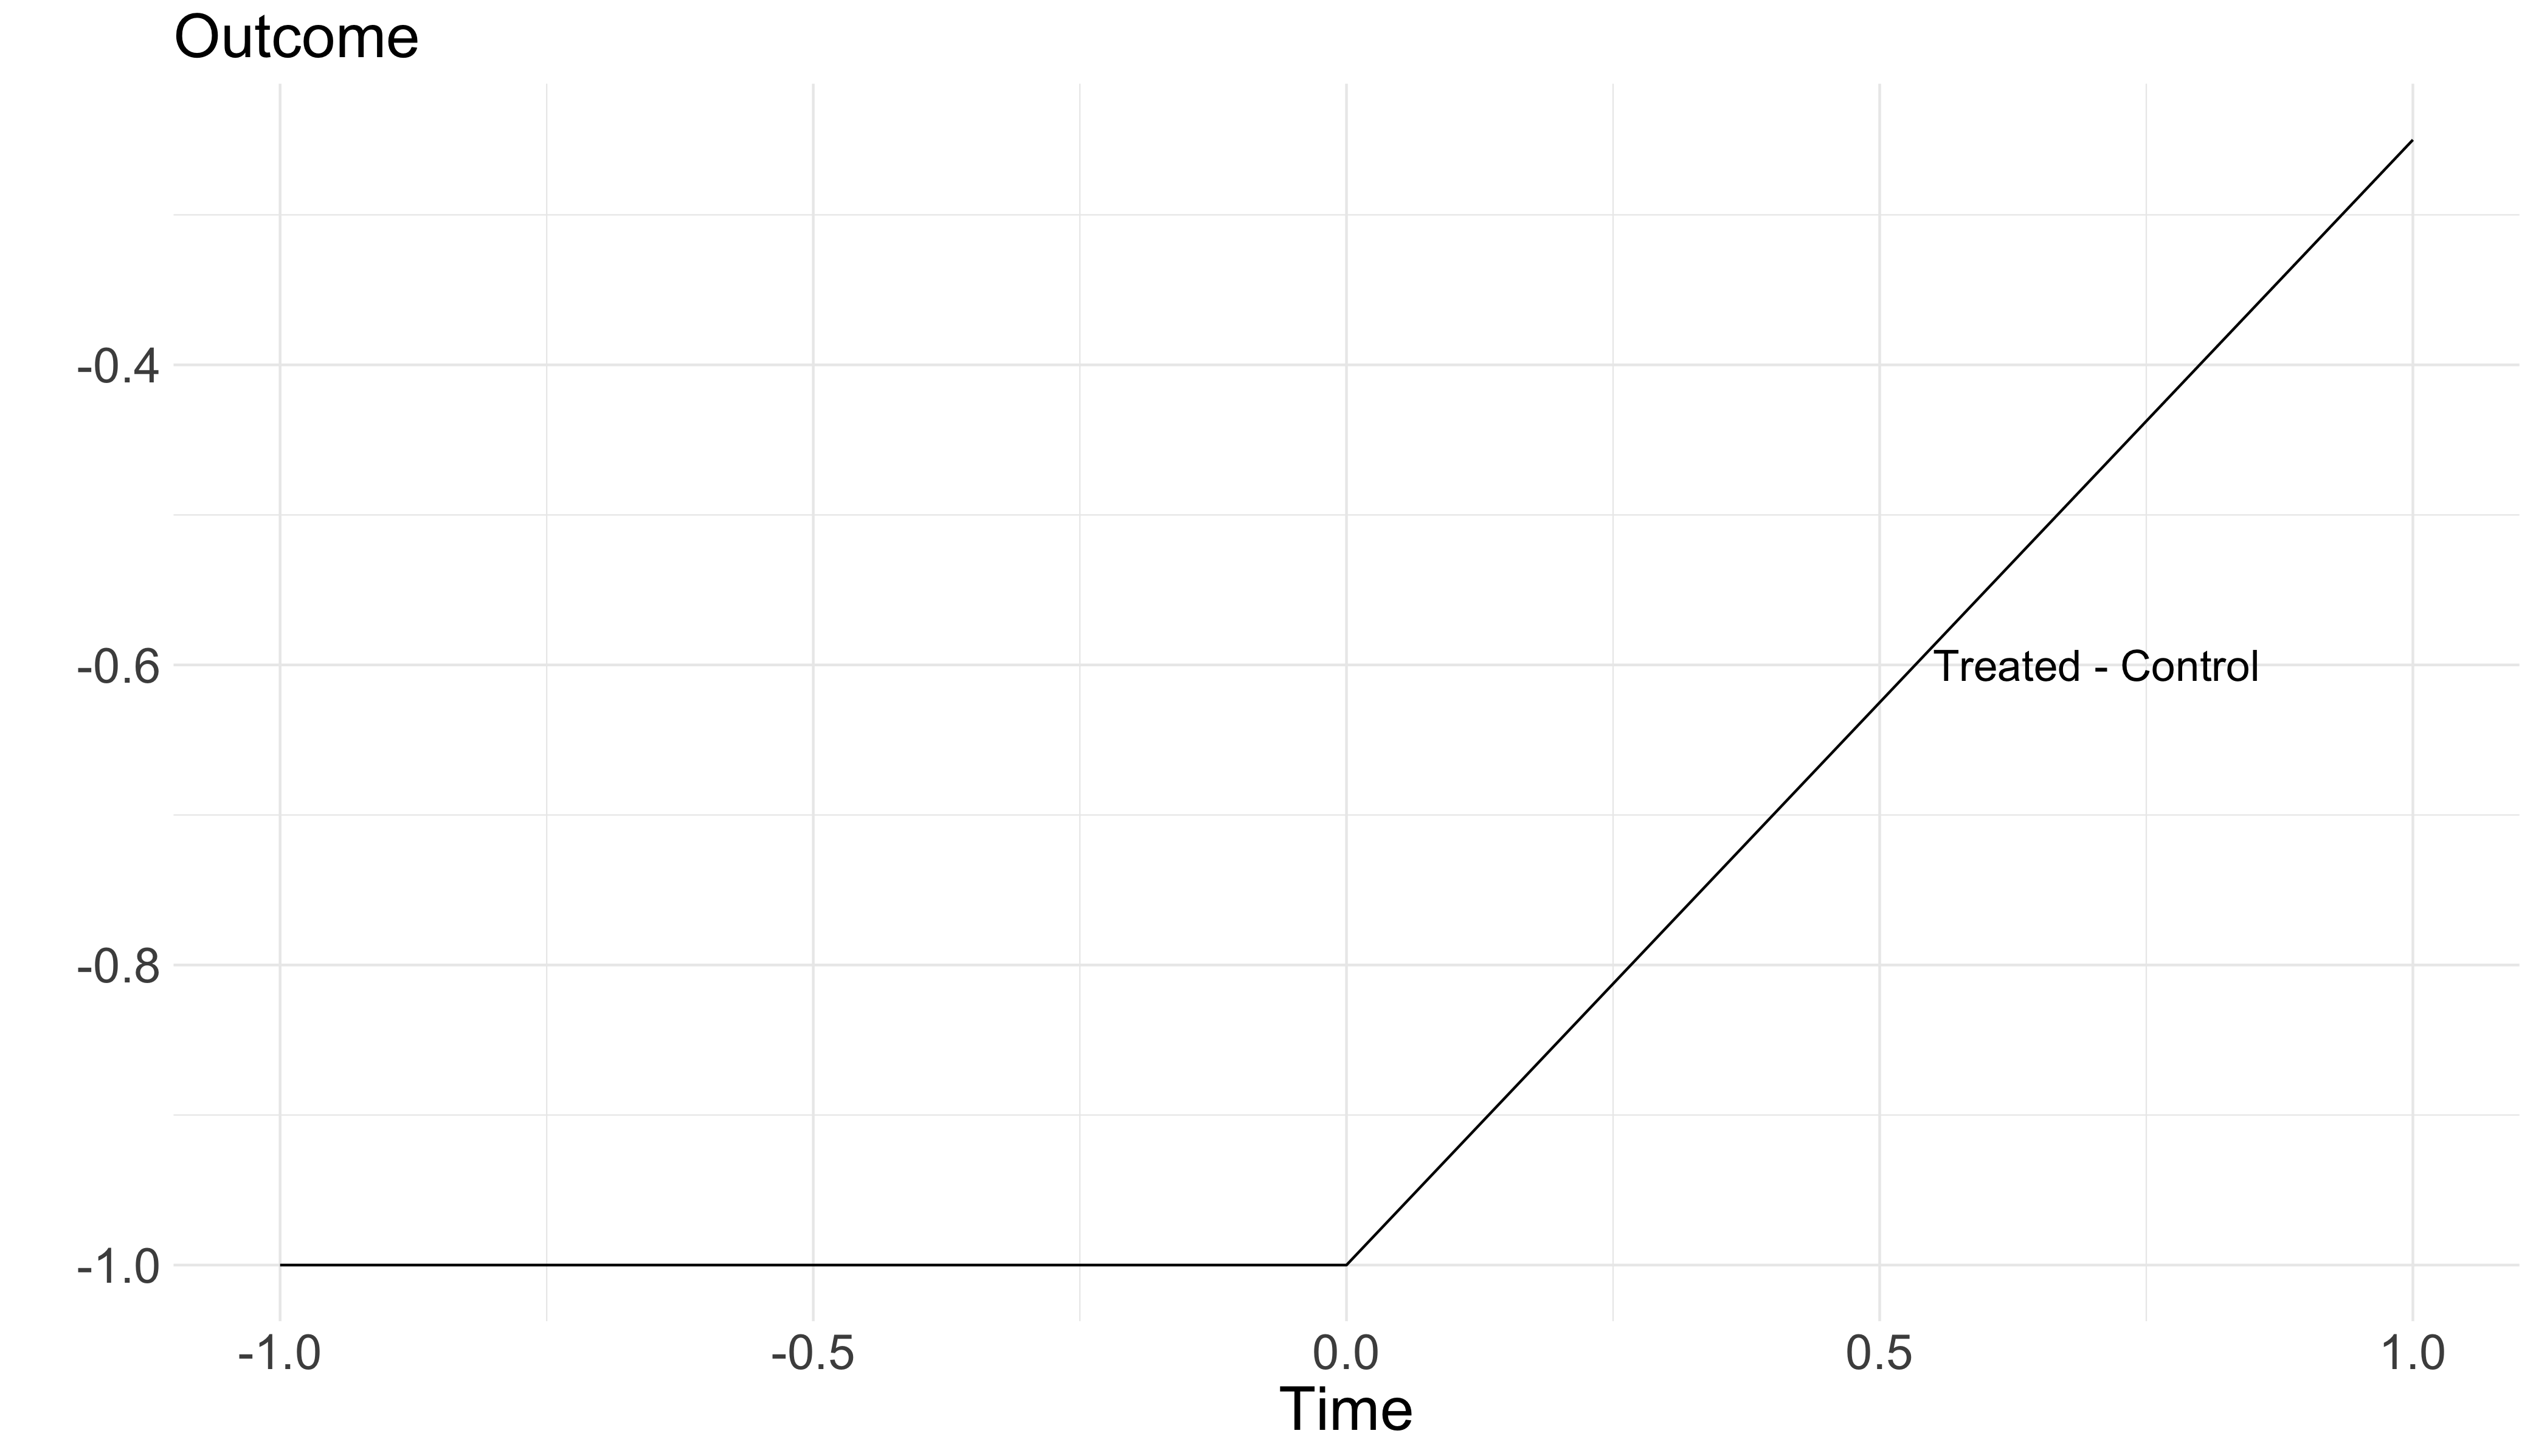
\includegraphics[width=\linewidth]{images/rothpic2.png}}
			\only<3>{      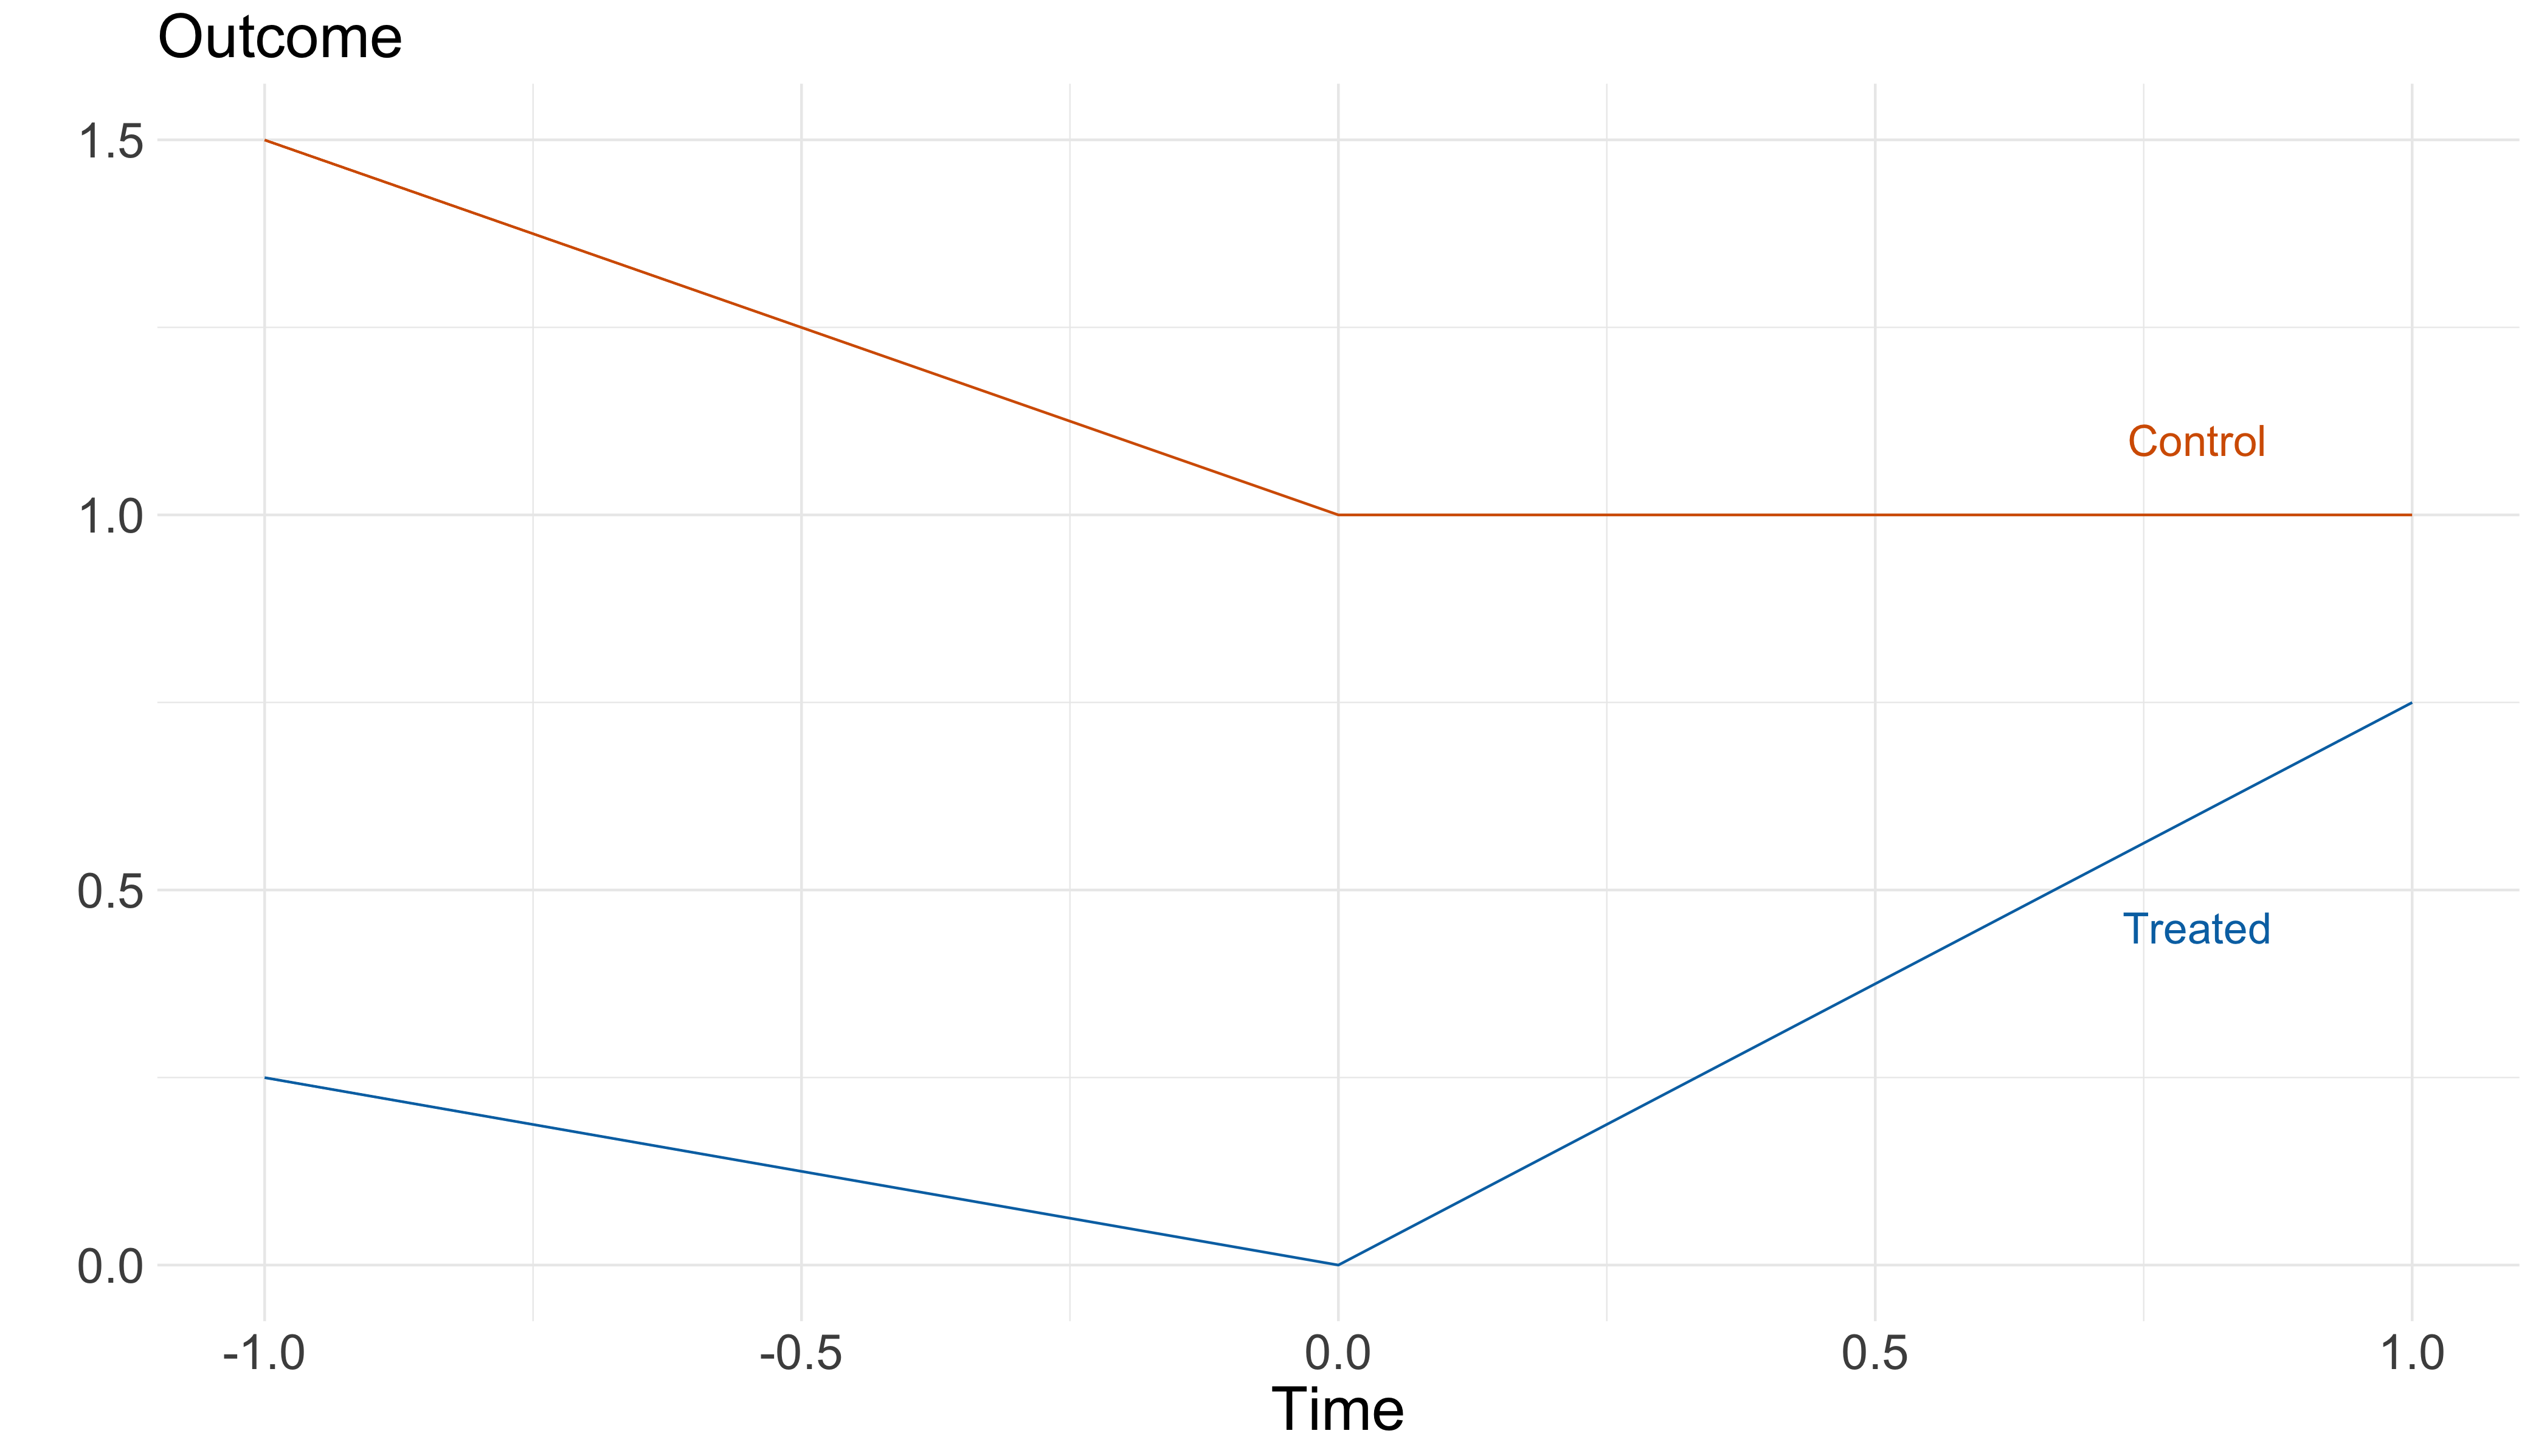
\includegraphics[width=\linewidth]{images/rothpic3.png}}
			\only<4>{      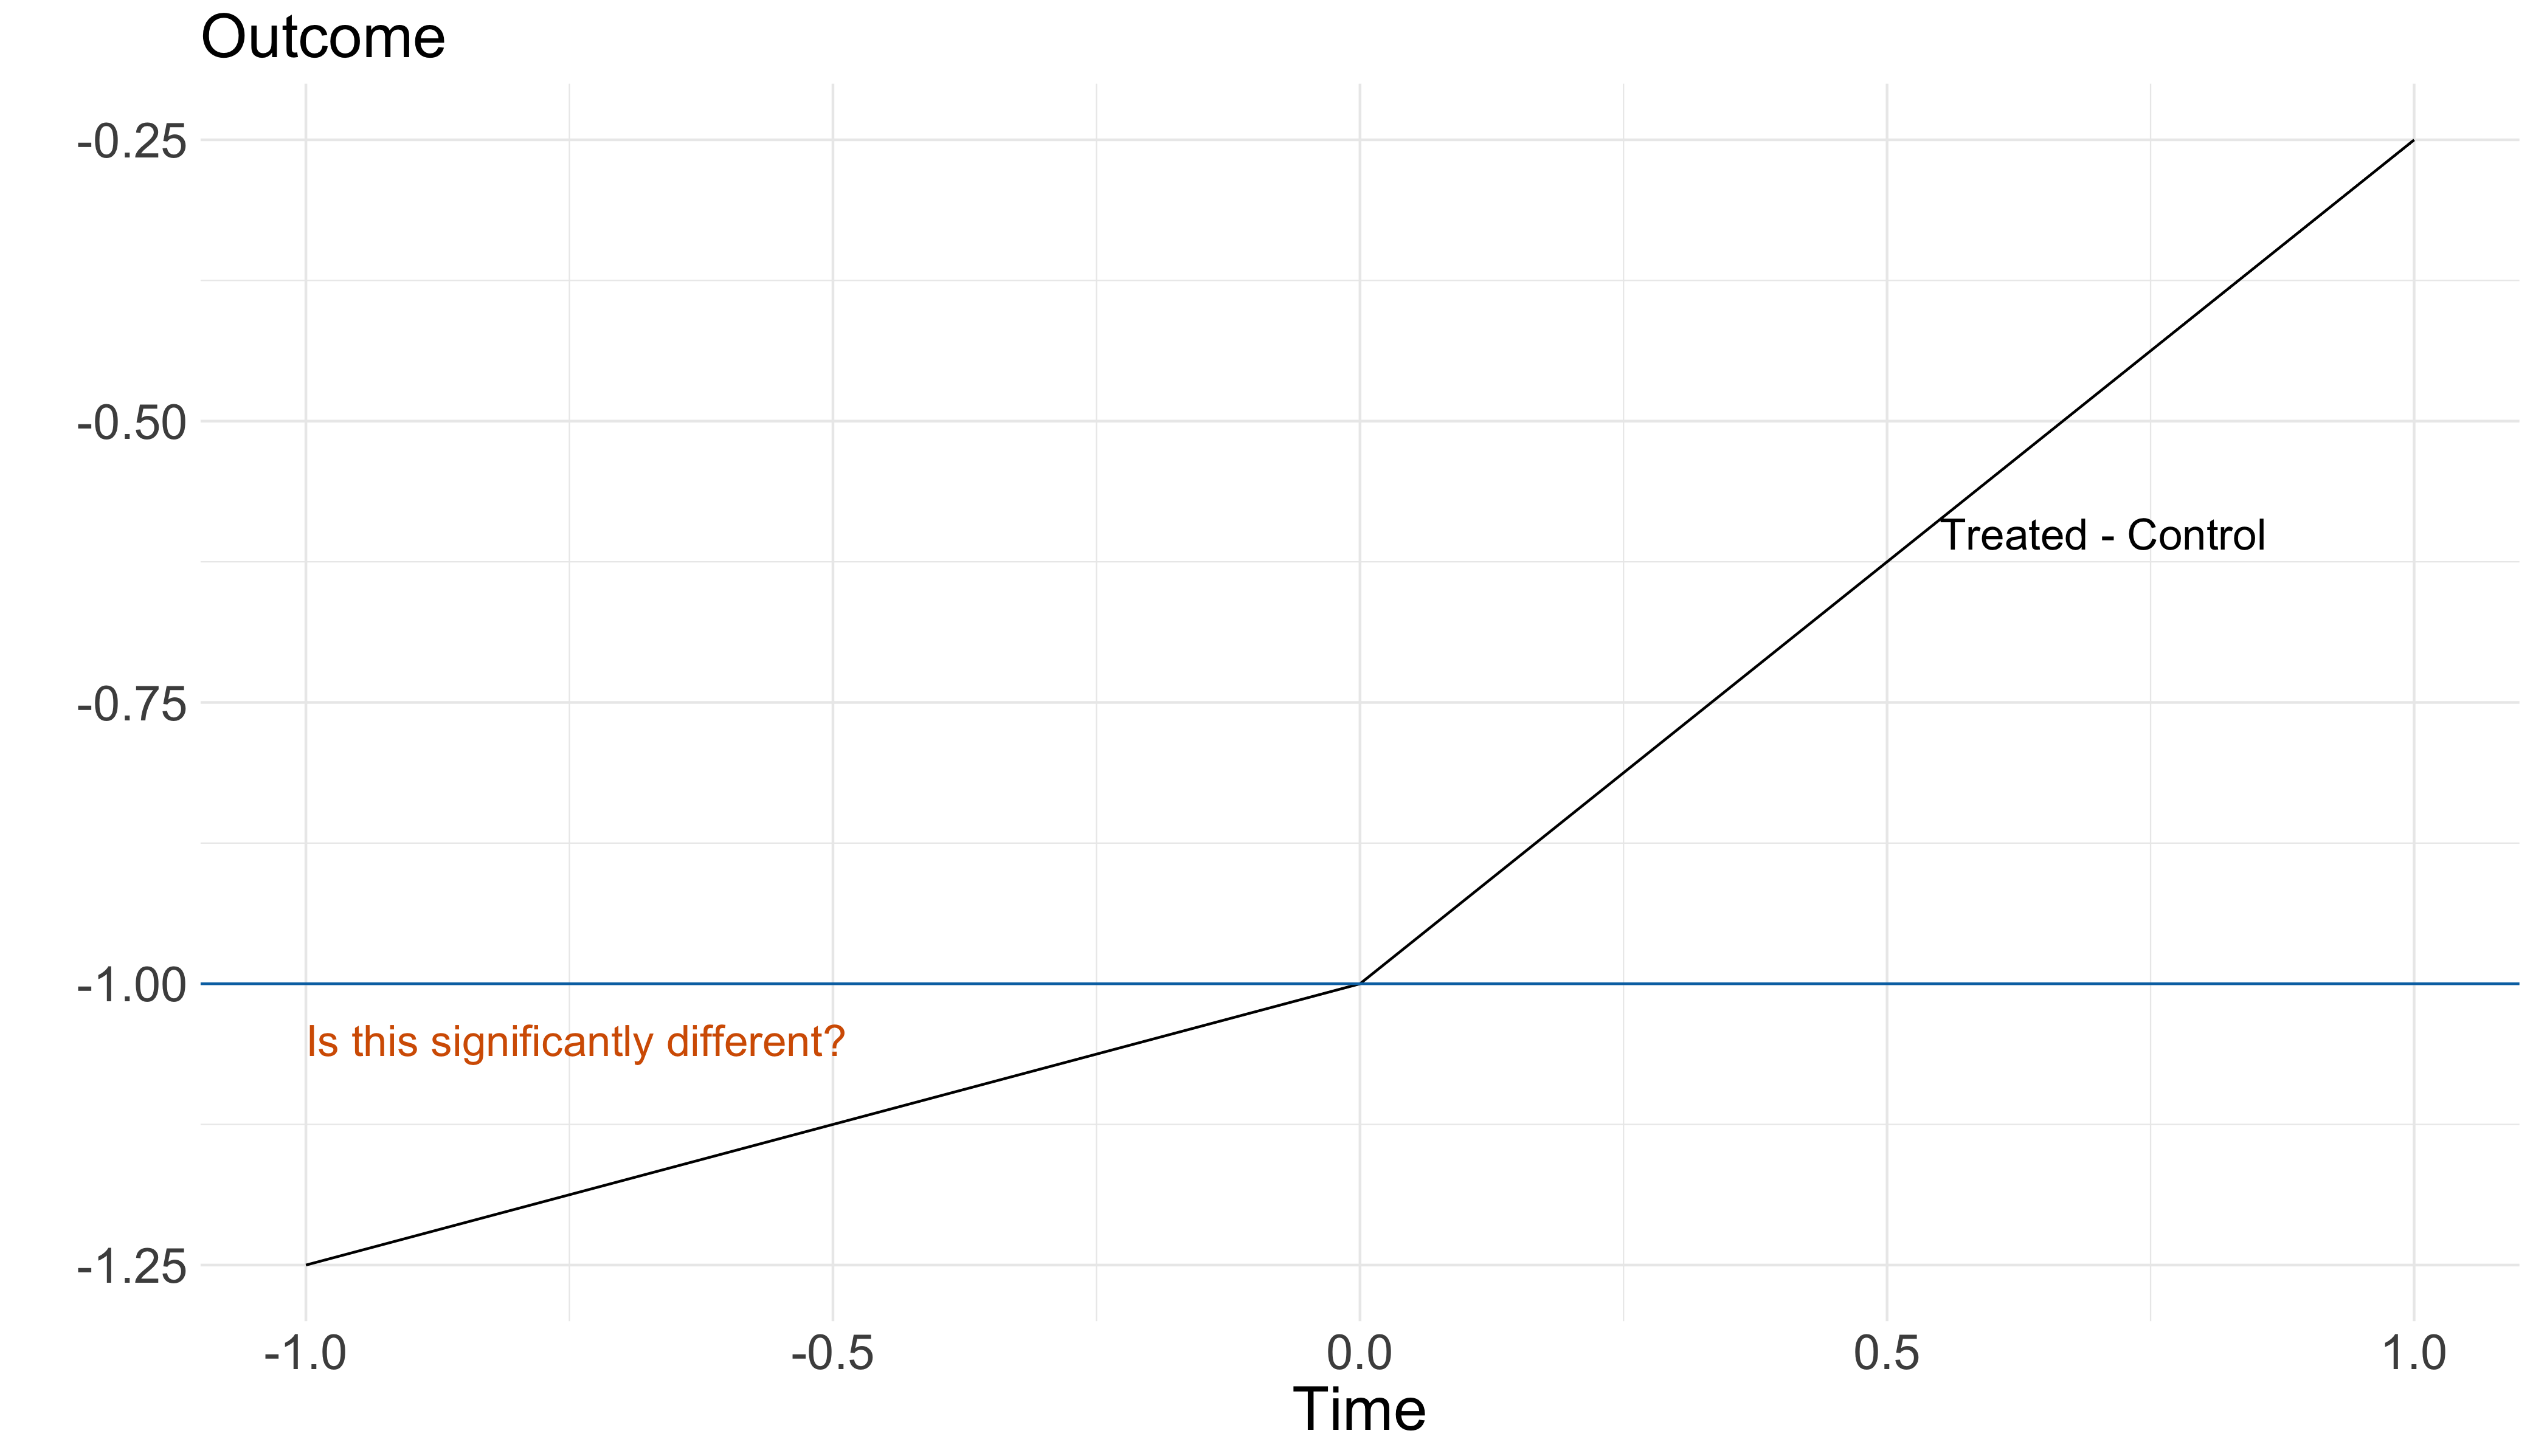
\includegraphics[width=\linewidth]{images/rothpic4.png}}
			\only<5>{      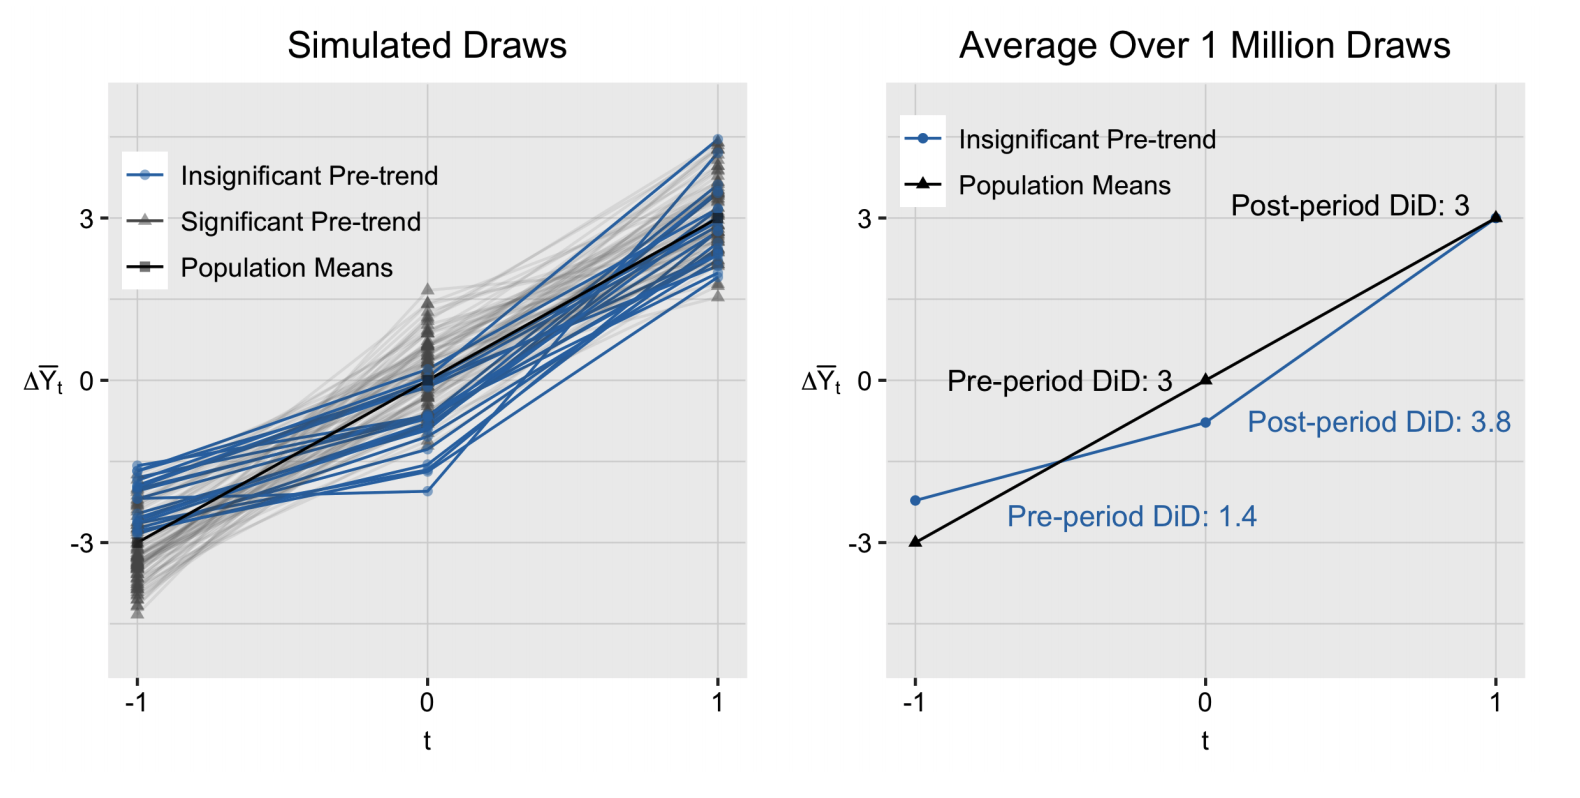
\includegraphics[width=\linewidth]{images/rothpic5.png}}
		\end{column}
	\end{columns}
\end{frame}

\begin{frame}{How to interpret this caution?}
	\begin{wideitemize}
		\item First, don't panic. Examining pre-trend is still important
		diagnostic
		\item Important to realize that selecting your design based on
		pre-trend is \emph{constructing} your counterfactual
		\begin{itemize}
			\item Pre-tests will cause you to potentially contaminate your
			      design
		\end{itemize}
		\item Suggested solution from Roth (2020): incorporate robustness to
		pre-trends into your analysis. Rambachan and Roth (2020) present
		results on testing sensitivity of DinD results to pre-trends
		\begin{itemize}
			\item Brief intuition follows
		\end{itemize}
	\end{wideitemize}
\end{frame}


\begin{frame}{Rambachan and Roth (2020) suggestion}
	\begin{wideitemize}
		\item Intuitive proposed solution for robustness. Note the post and pre effects:
		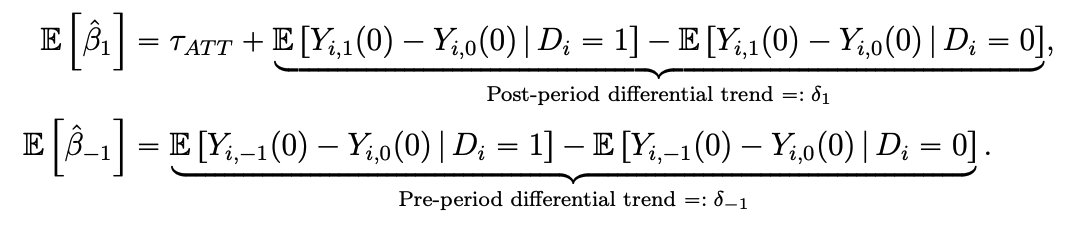
\includegraphics[width=0.7\linewidth]{images/rothpic6.png}
		\vspace{-10pt}
		\item parallel trends assumes these $\delta$ are zero. But pre-trends may not be zero.
		\begin{itemize}
			\item R\&R say: we can use the info from our pre-trends to bound
			      post-trend
			\item Use a \emph{smoothness} assumption, $M$, on the second derivative. E.g. simple case:
		\end{itemize}
		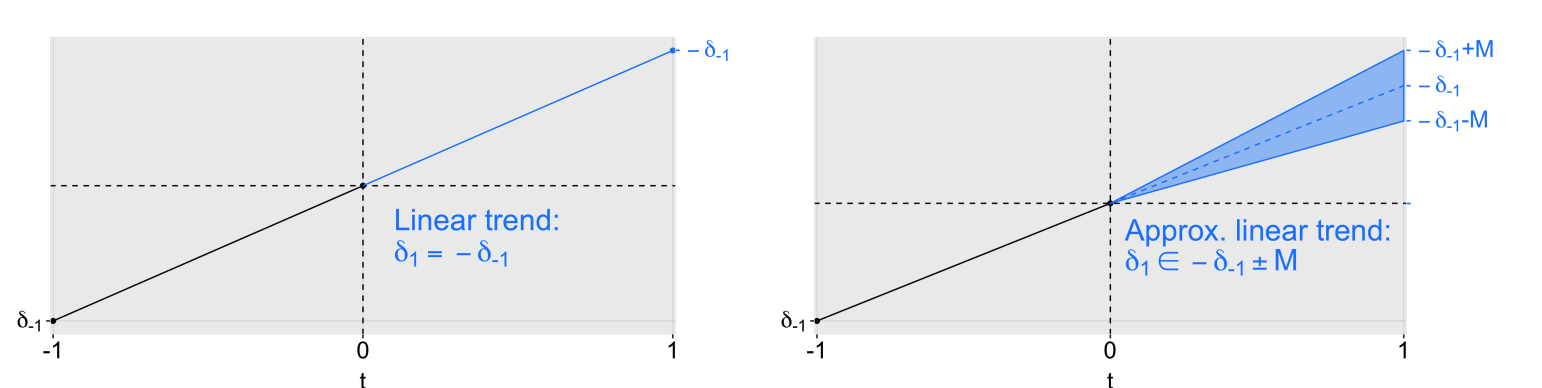
\includegraphics[width=\linewidth]{images/rothpic7.png}
	\end{wideitemize}
\end{frame}

\begin{frame}{This approach adds more work but also more validity}
	\begin{wideitemize}
		\item  Need to select $M$, and will likely have less strong results
		\item However, very powerful way to address concerns about pre-trends
		\item Code for applying this technique is availabe in R:
		\url{https://github.com/asheshrambachan/HonestDiD}
	\end{wideitemize}
\end{frame}

\begin{frame}{Parallel trends in what?}
	\begin{wideitemize}
		\item A known issue that was historically not formalized is the
		question of what the outcome is specified as: logs, or levels?
		\item Hopefully it's clear that if something satisfies pre-trends in
		logs, it seems unlikely to satisfy in levels
		\item Recall that this is the issue of \emph{invariance} we
		discussed with quantile treatment effects
		\begin{itemize}
			\item In our parametric setting, if there are time trends in the
			      outcomes, the parallel trends are likely not to hold for all
			      transformations of the variables.
			\item That could be problematic if you wanted to be agnostic about
			      the model!
		\end{itemize}
		\item Roth and Sant'Anna (2021) directly discuss this issue. Their suggestion:
		\begin{quote}
			Our results suggest that researchers who wish to point-identify
			the ATT should justify one of the following: (i) why treatment
			is as-if randomly assigned, (ii) why the chosen functional form
			is correct at the exclusion of others, or (iii) a method for
			inferring the entire counterfactual distribution of untreated
			potential outcomes.
		\end{quote}
	\end{wideitemize}
\end{frame}

\begin{frame}{Finally, a discussion on inference}
	\begin{wideitemize}
		\item First, let's start with the old school fact that you must know
		if you are working with panel data and Dind
		\item \textbf{You must cluster on the unit of policy implementation
			if possible}. See Bertrand, Duflo and Mullainathan (2004)
		\begin{itemize}
			\item Why? Outcomes and the treatment tend to be severely
			      autocorrelated within unit
			\item I say ``if possible'' since clearly in Card and Krueger that
			      is infeasible
		\end{itemize}
		\item If the policy variation is implemented at the industry level,
		you should not cluster at the firm level
		\item If the policy variation is implemented at the firm level, you
		cannot use robust standard errors
	\end{wideitemize}
\end{frame}

\begin{frame}{Small clusters}
	\begin{wideitemize}
		\item The Card and Krueger case was too extreme, but there are approaches for dealing with a small number of clusters
		\item This approach typically involves  bootstrapping, and can handle small number of treated groups relative to the overall population
		\item See Andreas Hagemann's work for a place to start
	\end{wideitemize}
\end{frame}

\begin{frame}{Uniform confidence intervals}
	\begin{wideitemize}
		\item Finally, when considering event study graphs, pre-trend graphs
		should use uniform confidence intervals, rather than pointwise confidence intervals
		\begin{itemize}
			\item Advocated for by Freyaldenhoven et al (2018):
		\end{itemize}
		\item Code available here thanks to Ryan Kessler: \url{https://github.com/paulgp/simultaneous_confidence_bands}
		\begin{center}
			\only<1>{    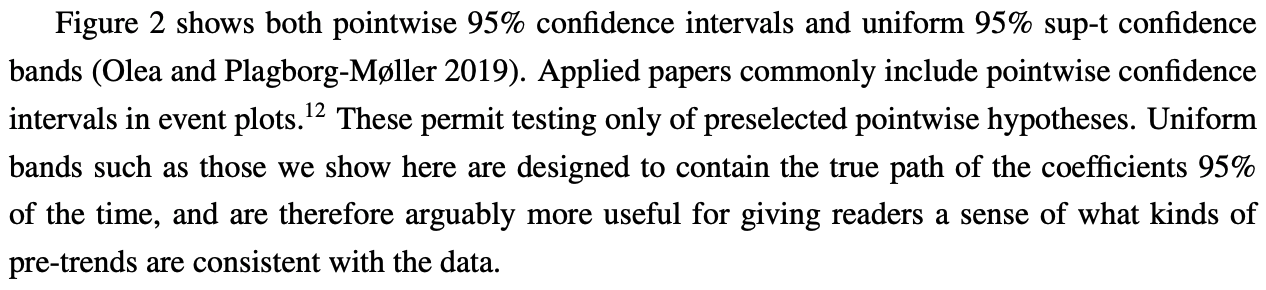
\includegraphics[width=\linewidth]{images/freyaldenhoven1.png}}
			\only<2>{    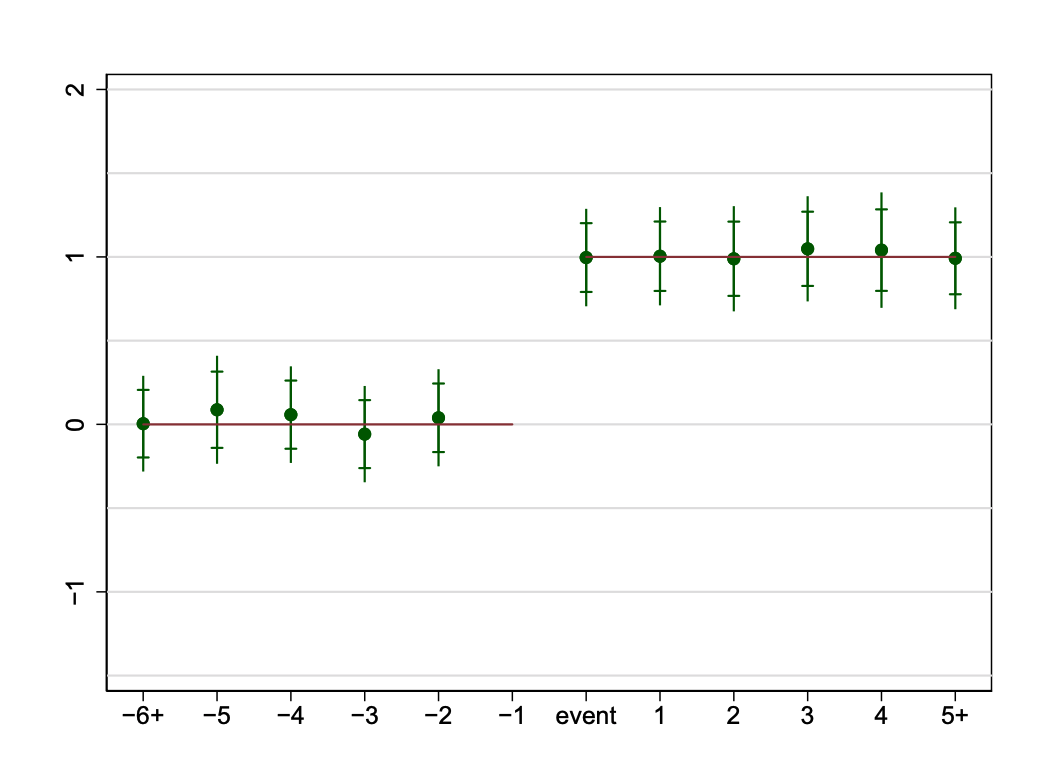
\includegraphics[width=0.5\linewidth]{images/freyaldenhoven2.png}}
		\end{center}
	\end{wideitemize}
\end{frame}

\begin{frame}{Takeaways}
	\begin{wideitemize}
		\item Difference-in-differences identifies causal effects using parallel trends and no-anticipation assumptions
		\item The 2x2 case is clean and intuitive --- multiple time periods let you partially test assumptions
		\item Beware weak tests of pre-trends. Consider using Rambachan and Roth's sensitivity analysis
		\item Parallel trends in logs vs. levels is a real concern --- think about functional form
		\item You must cluster on the unit of policy implementation
		\item Next class: what happens with staggered timing?
	\end{wideitemize}
\end{frame}

\end{document}
